\documentclass[12pt]{comjnl}

\usepackage{amsmath}

%\copyrightyear{2009} \vol{00} \issue{0} \DOI{000}
\linespread{1.5}

\begin{document}

\title[Hashtag Segmentation of Conversational Tweets in Turkish]{Hashtag Segmentation of Conversational Tweets in Turkish, Modelling Segmentation Approach Midterm Report}
\author{Ass. Prof. Arzucan Ozgur, Utku Saridede, Sevket Topuz}
\affiliation{Informational Retrival and Natural Language Processing, Department of
Computer Engineering, Bogazici University, Istanbul
Bebek 34342, TR} \email{utku.saridede@boun.edu.tr, sevket.topuz@boun.edu.tr}

\shortauthors{Saridede, Topuz}

\received{07 October 2015}
\revised{13 November 2015}

\keywords{Twitter; Tweets; Tweet; Hashtag; Segmentation; Turkish; Conversational Tweets;
		Hashtag Segmentation}

\begin{abstract}
Twitter is the latest social networking tool which affects everything related to the person.
Twitter allows its users to write at most 140 character long update, it is known off as 
``tweet''. In this research, analyzing segmentation of tweets is our main objective. There are
several researches in English, but not that much in Turkish. Studying with the Turkish corpus is
somehow hard to handle, because Turkish resources are insufficient. The usage of the hashtags
differ in country to country, that is, some countries do not know off proper usage of hashtags.
Having more than one word in the hashtag or lapsus calami are misusage, and prevent researchers 
to work properly. The other part of the project is analyzing hashtags in the way of linguistics.
Analyzed corpus will give more information about related countries. In the other words, short-term
hashtag analyses keep informed about spesific situations which influence the society. After all said
and done, we will recognize the strength of computer science on natural languages.
\end{abstract}

\maketitle

\section{Introduction}
A hashtag is defined by any string prefixed with a ``\#'', for instance, “\#freedomtomark”,
“\#shesuggest”. The string can be a single word, an acronym, or multiple words joined
together, and usually identifies the subject topic of the tweet (e.g., “\#ENG493”)
or expresses a comment about it (e.g., “\#kappamevku”). 

The main objective is to implement machine learning based hashtag segmentation application.
The first work was using twitter developer tools to 
extract tweets from their database. In the case of hashtag extraction, there are several issues. For instance,
we have recognized that Turkish people do not understand the usage of hashtag approach.
Therefore, the formation of corpus becomes difficult. Using large amount of raw data that 
is recieved from social media is the way of creating corpus. In the field of natural language 
processing, the essential requirements are datasets. Having realiable training and test data helps to improve
current algorithm. Because languages are flexible and few training and test data cause to 
reproduce wrong idea. It clarifies why there is not enough
research in Turkish. That is because, improving datasets might help researchers to test their idea and
models.

The starting point of project is primarily based upon gathering data to avoid
backing to drawing point. That is, being blind to quantity of data causes to quit idea.
Existing methods of word segmentation unsuperwised language models. Researches claim that
using multiple corpora, the joint probability model from multiple corpora performs significantly 
better than the individual corpora. Weighted joint probability model with weights is specific to each corpus. Decent approach is to train the weights in a supervised manner using max-margin methods, that is, a machine learning method to make a decision about the boundries of words.
The supervised probability models improve segmentation accuracy over joint probability models. 
Researchers observe that length of segments is an important parameter for word segmentation, and 
incorporating length-specific weights into our model supports the current model.
However the length specific models further improve segmentation accuracy over supervised 
probability models.

All mentioned models try to solve the problems with dynamic programming algorithms. The supervised length specific models have significantly more advencement over unsupervised single corpus and joint probability models. Segmentation of hashtags result in significant improvement in recall on searches for twitter trends.

The machine learning side of the computer science aims to investigate human related behaviours by definition. Computers should be able to learn how to analyze data from background information. There are similar researches about segmentation of sentences, and especially non-spaced words. The motivation of project comes from URL segmentation. URL segmentation brings same study to mind with the
evoluation of technology. The changes in the social media trends lead to extended works. The amount of Web page links are like god's creatures. That is, Web has a link inheritance that is increasing over time. Collecting data from Web links is somehow stable. However, hashtag case needs some time to be imporved and had data inheritance.

\section{State of Art}

Word segmentation are of great interest to Natural Language Processing researchers. 
A good number of methods have been proposed in the literature, with quite good 
performances reported. There are several articles about word segmentation. 
There are two major categories, as well as, boundary prediction and word 
recognition. One of the most frequently used method
for that is maximum matching, by Wong and Chan – 1996. Many approaches help us to handle
unknown words and to get best proper answer in the case of ambiguity.

Boundary prediction methods usually used with local statistics
to decide the boundary between two language units located in local store. The representative
examples involve Ando-Lee Criterion (Ando and Lee 2000),
Mutual Information (Sun, Shen, and Tsou 1998) and
Branching Entropy (Jin and Tanaka-Ishii 2006). Fleck (2008) built an algorithm called
WordEnds. It became a boundary classifier with the dixit
boundary clues, then used it to mark word boundaries.
Zhikov, Takamura, and Okumura (2010) buit
an powerful algorithm combining the strength of Minimum
Description Length review and local statistics Branching Entropy.
High performance in the case of accuracy and speed had been seen.

Seperating a string into different words is not a simple task to be done automatically. Some people capitalize the first letter of each word. Other use underscores to split owrds. However, using underscores is waste characters. Users usually write without any evident or coherent use of separation signs and there are no known rules to rely on segmenting hastags.

Another approach is word segmentation of URL links. To think about the word segmentation and
recognition problem for URL links, reasearchers adopt some basic principles from rule­based
approach. The dictionary should have sufficient amount of word entries. However, the occurence
of compound words makes it very difficult to match every component string exactly with the
dictionary entries. Evaluation of the hashtag segmentation has started to be improved with search engine
improvements of Twitter.

\begin{figure}
\centering
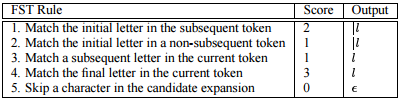
\includegraphics[width=3.5in]{method.png}
\caption{Example of title token based finite state transducer (FST). Explanation of the use of hashtag segmentation and text quality ranking. Rules for the title expansion.}\label{fig:Tweet}
\end{figure}

Finite state transducer is an approach for title token base URL segmentation. It splits and segments according to previous-seen web page title simultaneously. For example, URL link includes "cs" that might correspond to "computer science" in many training page's title. If "cs" is encountered in the testing corpus, it is automatically expanded to "computer science". The tranducer has several rules that give score. This score can be obtain by certain moves which match or skip letters in the tokens of title with corresponding letters. Expansion can be valid if it covers all letters in the segment.

\section{Methods}
We have tried to discourse manly with 3 methods. Hashtag segmentation can be generally defined as word boundry detection. Because of this, we
start with detection of the word boundry. There are two feature­based learning methods,
Conditional Random Fields (CRFs)(Laerty et al.,2001) and Maximum Entropy (MaxEnt).
CRFs can represent the uncommon parts of the information as elements furthermore, are great at
displaying grouping marking problems. MaxEnt is extremely compelling at learning with a high
assortment of components, without agonizing over the multifaceted nature of the model. Hidden
Markov Model is a simplistic approach for word segmentation. It helps us to built character
trigrams. It tries to catch boundary characters that are current and previous ones. Peter Norvig's
implementation can be used for word bigrams.

Manual annotation is time consuming task and it limits the amount of trainig data that can be
created. We try to achieve utilizing data to create training sets for hashtag segmentation. Synthetic
hashtags by concatenating the words in tweets can also be used for training data because word
boundries are known. To use concatenating the words in tweets as training dataset, we need to filter
non­word tokens. If tweets include non­word token in the beginnig or end of the text, it can be
removed and other words can be used as trainig data. On the other side, if a non­word token appear
in the middle of the text, the tweet is dicarded because non­word token ib the middle of the tweet
may distort the word order. The word order is important point of trainig data.

Word boundry detectiton and word segmentation is very important for Chinese words segmentation. A good research about Chinese word segmentation can be found out in Wu and Tseng's paper. A Chinese senteces do not
include delimiters to seperate words. It includes combined of a string of characters. Netural
networks and lazy learning (just-in-time learning) approaches are methods that are used in word segmentation.
Processing of the examples are collected until a clear request for information is received. When the information recieved, the databse search is completed according to amount of the distance that is most related to query.

We can use each character of training data to represent one function of learning system. Some
features should be determined and each character should be examined according to these features
to create machine learning system.

\section{Results}
We have collected the tweets from twitter. We tokenize tweets, normalize them and get 
hashtags from them. We have stored all information related to tweets. That will help us to recognize training and test data. The training data will be the part of the current data.

\begin{figure}
\centering
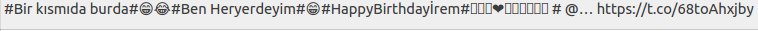
\includegraphics[width=3.5in]{tweet.png}
\caption{Tweet example.}\label{fig:Tweet}
\end{figure}

Implementing a method to get hashtags and insert them database is 
accomplished. There are two kind of table as well as "TEXTS" which contains unique tweet IDs
and tweet text.

\begin{figure}
\centering
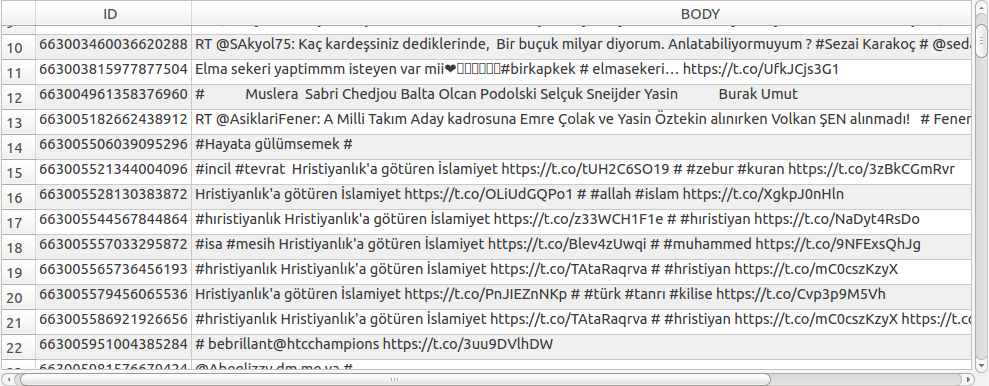
\includegraphics[width=3.5in]{text.png}
\caption{Text database table representation.}\label{fig:Tweet}
\end{figure}

The other one is "HASHTAGS" which contains tweet IDs and hashtags. Segmentation algorithm
is almost done.

\begin{figure}
\centering
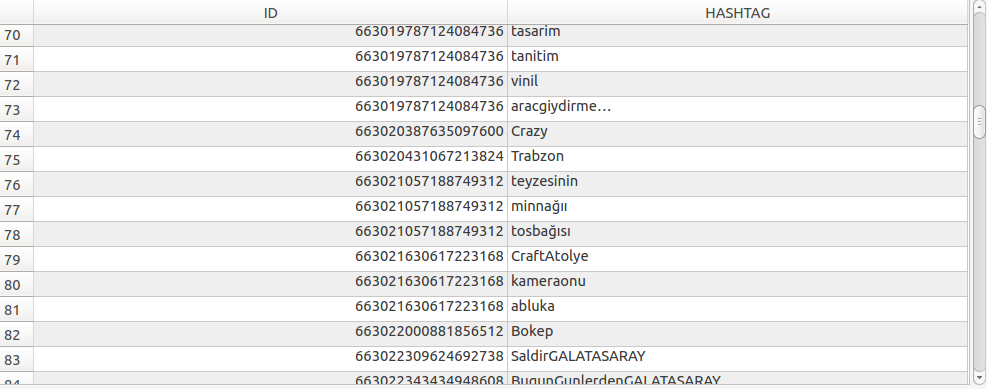
\includegraphics[width=3.5in]{hashtag.png}
\caption{Hashtag database table representation.}\label{fig:Hashtag}
\end{figure}

\section{Conclusion}
We proposed a simple and effective unsupervised
word segmentation approach. The criterion incorporates
boundary information to model words.

\section{Future Work}
We decided to improve our segmentation algorithm. Features of the words will be dicussed. Training and test
datasets will be prepared. Every word in the training data will be used to improve machine
learning power of our project. Later future works will be consulted to Prof. OZGUR.

\section{References}
- Berardi, Giacomo; Esuli, Andrea; Marcheggiani, Diego and Sebastiani, Fabrizio. Exploring the use of hashtag segmentation and text quality ranking 
Istituto di Scienza e Tecnologie dell’Informazione Consiglio Nazionale delle Ricerche 56124 Pisa, Italy

- Kan, Min-Yen, Web Page Classification

- Bansal, P., Bansal, R. and Varma V. 2015. Towards
Deep Semantic Analysis Of Hashtags.

- Berardi, G. and Esuli, A. and Marcheggiani, D. and
Sebastian, F. 2011. ISTI@TREC Microblog track
2011: exploring the use of hashtag segmentation
and text quality ranking.

- Chen, S. and Xu Y. and Chang, H. 2012. A Sim-
ple and Effective Unsupervised Word Segmentation
Approach. Proceedings of the Twenty-Fifth AAAI
Conference on Artificial Intelligence

- Xue, N. 2003. Chinese word segmentation as charac-
ter tagging.. International Journal of Computational
Linguistics and Chinese Language Processing vol-
ume 8(1)

- Wong, P and Chan, C. 1996. Chinese word segmenta-
tion based on maximum matching and word binding
force.
\nocite{*}

\bibliographystyle{compj}
\bibliography{ModellingBidders}


\end{document}